\chapter{Παρουσίαση Αποτελεσμάτων}
\label{ch:chapter3}

\section{Ερώτημα 1}

Όλα τα παρακάτω γραφήματα αφορούν τη μέθοδο διχοτόμου.

\begin{figure}[H]
    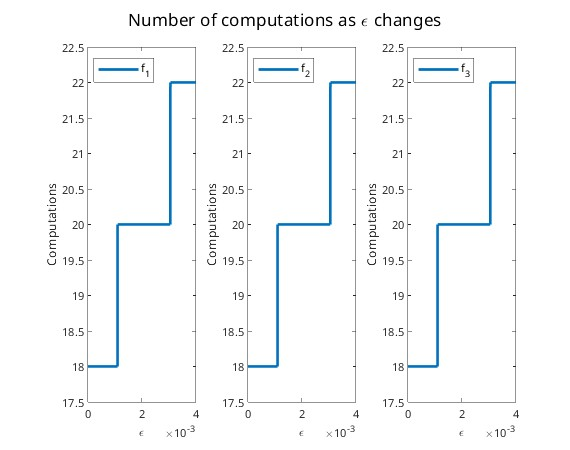
\includegraphics[scale=0.7]{plots/ex1/e_comps.jpg}
    \label{fig:funcs}
    \caption{Ο αριθμός των απαιτούμενων υπολογισμών ως συνάρτηση του $\epsilon$}
    \centering
\end{figure} 

\begin{figure}[H]
    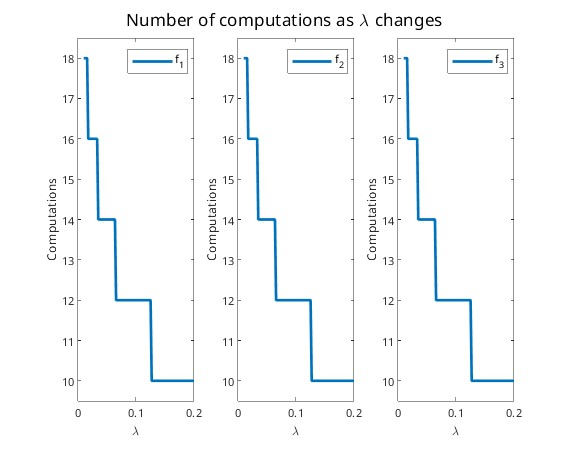
\includegraphics[scale=0.7]{plots/ex1/l_comps.jpg}
    \label{fig:funcs}
    \caption{Ο αριθμός των απαιτούμενων υπολογισμών ως συνάρτηση του $\lambda$}
    \centering
\end{figure}

\begin{figure}[H]
    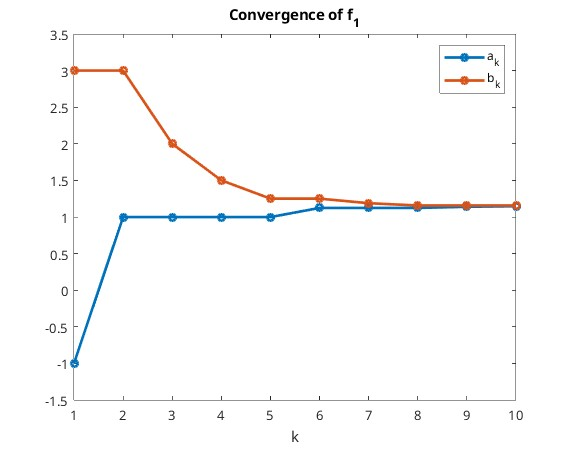
\includegraphics[scale=0.7]{plots/ex1/f1.jpg}
    \label{fig:funcs}
    \caption{Τα άκρα του διαστήματος $[\alpha, \beta]$ ως συνάρτηση του $k$ - $f_1$}
    \centering
\end{figure}

\begin{figure}[H]
    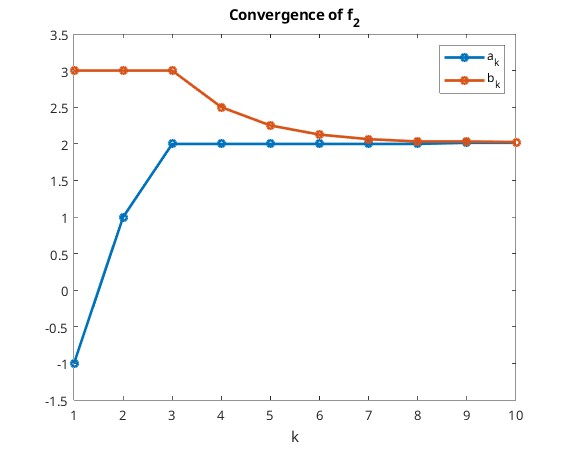
\includegraphics[scale=0.7]{plots/ex1/f2.jpg}
    \label{fig:funcs}
    \caption{Τα άκρα του διαστήματος $[\alpha, \beta]$ ως συνάρτηση του $k$ - $f_2$}
    \centering
\end{figure}

\begin{figure}[H]
    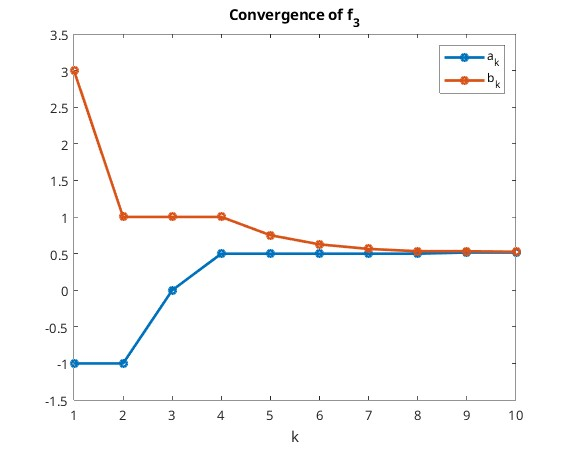
\includegraphics[scale=0.7]{plots/ex1/f3.jpg}
    \label{fig:funcs}
    \caption{Τα άκρα του διαστήματος $[\alpha, \beta]$ ως συνάρτηση του $k$ - $f_3$}
    \centering
\end{figure}

\section{Ερώτημα 2}

Όλα τα παρακάτω γραφήματα αφορούν τη μέθοδο χρυσής τομής.

\begin{figure}[H]
    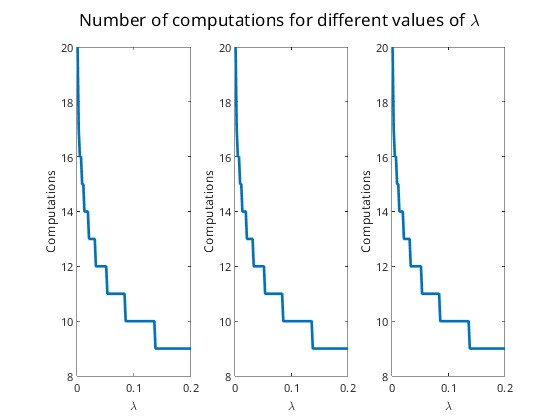
\includegraphics[scale=0.7]{plots/ex2/l_comps.jpg}
    \label{fig:funcs}
    \caption{Ο αριθμός των απαιτούμενων υπολογισμών ως συνάρτηση του $\lambda$}
    \centering
\end{figure}

\begin{figure}[H]
    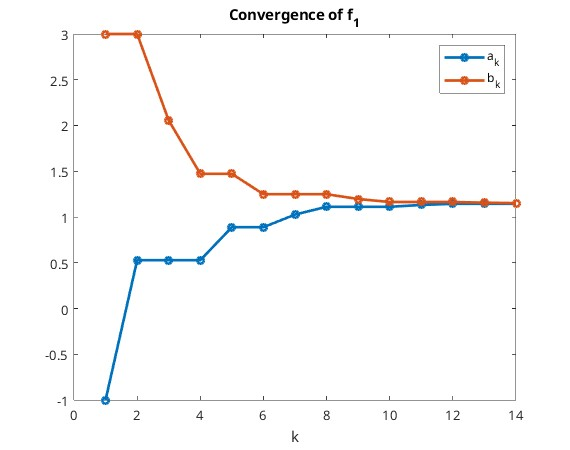
\includegraphics[scale=0.7]{plots/ex2/f1.jpg}
    \label{fig:funcs}
    \caption{Τα άκρα του διαστήματος $[\alpha, \beta]$ ως συνάρτηση του $k$ - $f_2$}
    \centering
\end{figure}

\begin{figure}[H]
    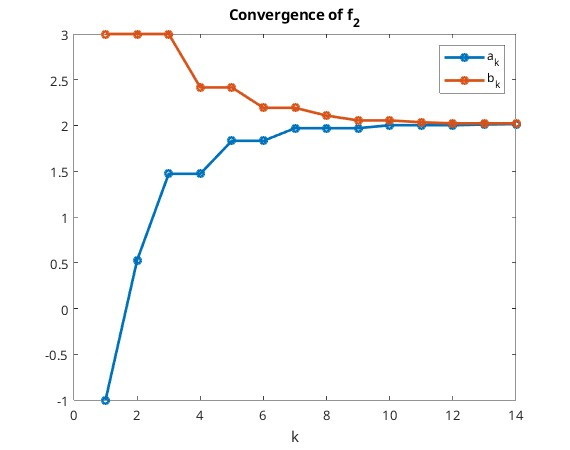
\includegraphics[scale=0.7]{plots/ex2/f2.jpg}
    \label{fig:funcs}
    \caption{Τα άκρα του διαστήματος $[\alpha, \beta]$ ως συνάρτηση του $k$ - $f_2$}
    \centering
\end{figure}

\begin{figure}[H]
    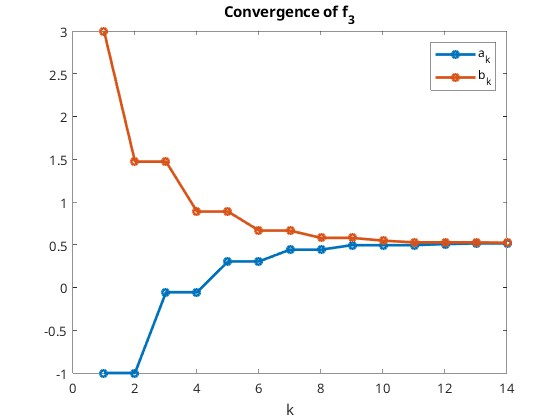
\includegraphics[scale=0.7]{plots/ex2/f3.jpg}
    \label{fig:funcs}
    \caption{Τα άκρα του διαστήματος $[\alpha, \beta]$ ως συνάρτηση του $k$ - $f_3$}
    \centering
\end{figure}

\section{Ερώτημα 3}

Όλα τα παρακάτω γραφήματα αφορούν τη μέθοδο \selectlanguage{english}Fibonacci\selectlanguage{greek}.

\begin{figure}[H]
    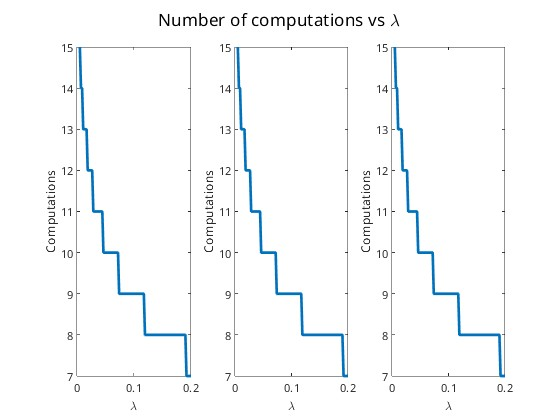
\includegraphics[scale=0.7]{plots/ex3/l_comps.jpg}
    \label{fig:funcs}
    \caption{Ο αριθμός των απαιτούμενων υπολογισμών ως συνάρτηση του $\lambda$}
    \centering
\end{figure}

\begin{figure}[H]
    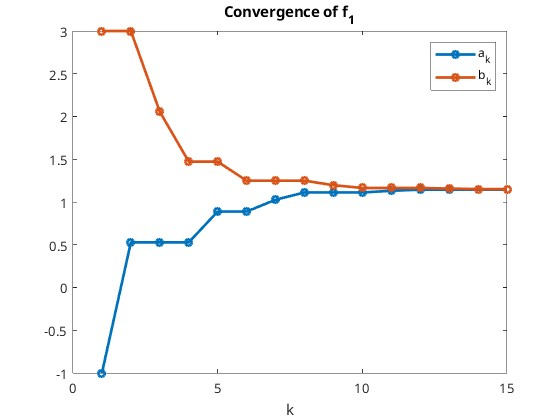
\includegraphics[scale=0.7]{plots/ex3/f1.jpg}
    \label{fig:funcs}
    \caption{Τα άκρα του διαστήματος $[\alpha, \beta]$ ως συνάρτηση του $k$ - $f_1$}
    \centering
\end{figure}

\begin{figure}[H]
    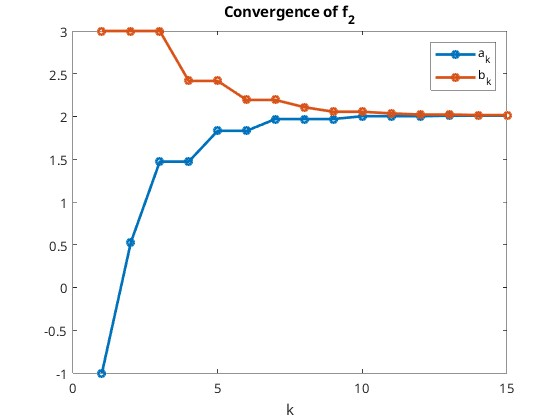
\includegraphics[scale=0.7]{plots/ex3/f2.jpg}
    \label{fig:funcs}
    \caption{Τα άκρα του διαστήματος $[\alpha, \beta]$ ως συνάρτηση του $k$ - $f_2$}
    \centering
\end{figure}

\begin{figure}[H]
    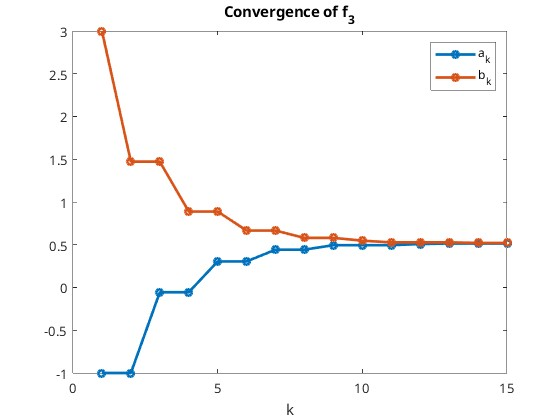
\includegraphics[scale=0.7]{plots/ex3/f3.jpg}
    \label{fig:funcs}
    \caption{Τα άκρα του διαστήματος $[\alpha, \beta]$ ως συνάρτηση του $k$ - $f_3$}
    \centering
\end{figure}

\section{Ερώτημα 4}

Όλα τα παρακάτω γραφήματα αφορούν τη μέθοδο διχοτόμου με χρήση παραγώγων.

\begin{figure}[H]
    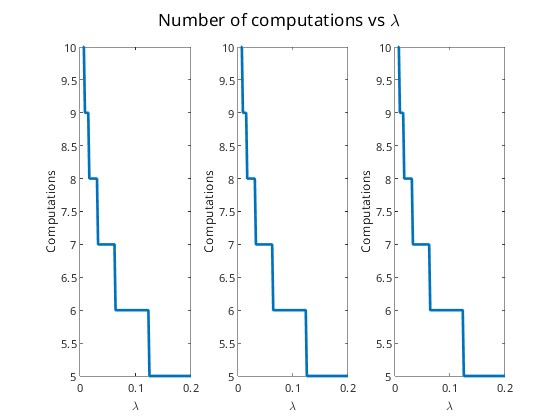
\includegraphics[scale=0.7]{plots/ex4/l_comps.jpg}
    \label{fig:funcs}
    \caption{Ο αριθμός των απαιτούμενων υπολογισμών ως συνάρτηση του $\lambda$}
    \centering
\end{figure}

\begin{figure}[H]
    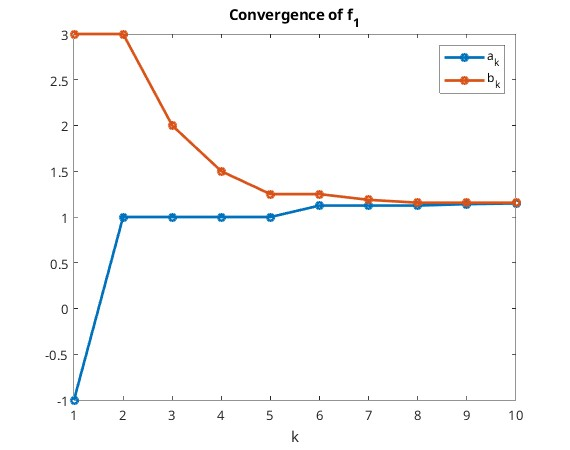
\includegraphics[scale=0.7]{plots/ex4/f1.jpg}
    \label{fig:funcs}
    \caption{Τα άκρα του διαστήματος $[\alpha, \beta]$ ως συνάρτηση του $k$ - $f_1$}
    \centering
\end{figure}

\begin{figure}[H]
    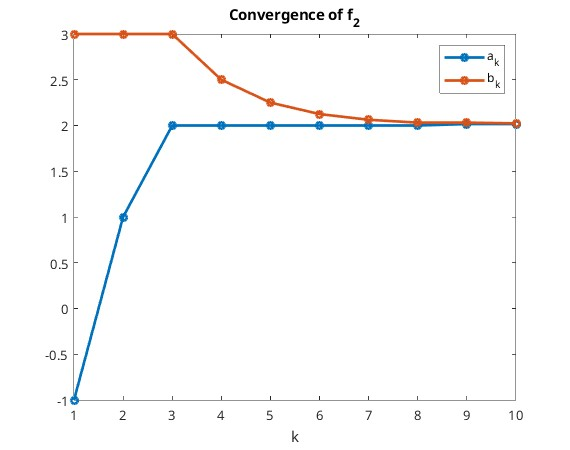
\includegraphics[scale=0.7]{plots/ex4/f2.jpg}
    \label{fig:funcs}
    \caption{Τα άκρα του διαστήματος $[\alpha, \beta]$ ως συνάρτηση του $k$ - $f_2$}
    \centering
\end{figure}

\begin{figure}[H]
    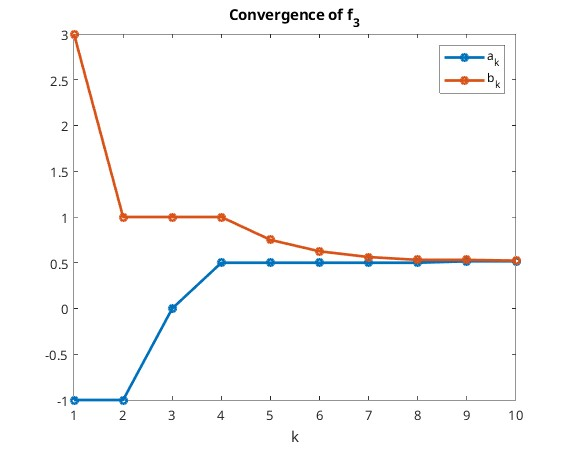
\includegraphics[scale=0.7]{plots/ex4/f3.jpg}
    \label{fig:funcs}
    \caption{Τα άκρα του διαστήματος $[\alpha, \beta]$ ως συνάρτηση του $k$ - $f_3$}
    \centering
\end{figure}